\begin{frame}{Verification Motivation}
\begin{itemize}
\item Smart contracts can manage a lot of money
\item The DAO attack costed around $60$\$ milion dollars
\begin{itemize}
\item Exploits re-entrancy vulnerability
\item Separation of the community: Ethereum Classic vs Ethereum
\end{itemize}
\end{itemize}

\begin{figure}
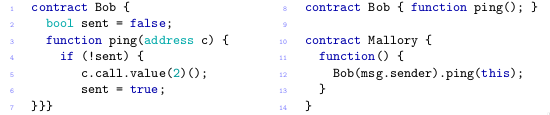
\includegraphics[width=0.9\textwidth]{./img/reentrancy}
\end{figure}

\begin{itemize}
\item Parity multiwallet signature
\begin{itemize}
\item Attackers "accidentally" \textbf{froze} $300$\$ milion dollars
\end{itemize}
\end{itemize}

\end{frame}

\begin{frame}{Common Bugs/Vulnerabilities \cite{bib:atzei,luu2016making}}
The majority of bugs are due to erroneous assumptions on the semantics of the EVM by developers
\begin{itemize}
\item Call to unknown
\item Mishandled Exception
\item Reentrancy
\item Transaction-ordering dependence (TOD)
\item Timestamp dependence
\item etc.
\end{itemize}

\end{frame}


\begin{frame}{Object of Verification}

\begin{block}{EVM}
\begin{itemize}
\pro It is stored on the blockchain
\pro gas consumption defined only for bytecode
\con Developers do not read bytecode
\end{itemize}
\end{block}

\begin{block}{Intermediate Language}
\begin{itemize}
\pro more high-level than bytecode
\con closer to bytecode wrt high-level language
\end{itemize}
\end{block}

\begin{block}{Solidity}
\begin{itemize}
\con Source code not necessarily public
\con Solidity change rapidly (still not 1.0)
\con Lack of formal specification
\pro Code readable by developers and auditors
\end{itemize}
\end{block}

\end{frame}

